\documentclass [12pt, a4paper] {article}
	\usepackage{float}
	\usepackage[utf8]{inputenc}
	\usepackage{amsmath}
	\usepackage{amssymb}
	\usepackage[russian]{babel}
	\usepackage[pdftex]{graphicx}
	\graphicspath{{pictures/}}
	\DeclareGraphicsExtensions{.pdf,.png,.jpg}
	\usepackage{amsthm}
	\usepackage{tikz}
	\usepackage{pgfplots}
	\usepackage{amsbsy}
	\usepackage{enumerate}
	\newtheorem{lemma}{Лемма}
	\theoremstyle{definition}
\begin{document}
	\section{Общая информация об обьекте наблюдения}
	Линзовидная галактика NGC7465. Координаты: $\alpha=23^{\circ} 02^{\prime} 16^{\prime \prime}.04$, $\delta = +15^{\circ}59^{\prime}33^{\prime \prime}.80$~(эпоха J2004.600). Дата наблюдений - 17.08.2004, время - 00:22:05. Детектор - EEV~CCD42-40, угловой масштаб пикселя - $0^{\prime \prime}.357\times0^{\prime \prime}.357$, размер матрицы - $1044\times1046$ пикселей. Наблюдения производились в фильтрах B, V, I, R. Для всех фильтров получены кадры обьектов, плоского поля и смещения. Кадров теневого тока нет, но температура матрицы при наблюдении (во всех фильтрах) порядка $150^\circ$K, поэтому теневым током можно принебречь.
	\section{Обработка данных}
	Из кадров экспозиции был вычтен кадр полученный усреденением всех кадров смещения, затем каждый кадр был поделен на кадр, полученный как медиана кадров плоского поля. На кадрах плоского поля присутствуют яркие точки (скорее всего соответсвующие ярким звездам), но они находятся вдали от области кадра, в которой находилась галактика, поэтому их наличие было проигнорировано. Затем полученные обработанные кадры экспозиции были совмещены и сложены. 
	При учете плоского поля в центре кадра ушли все видимые артефакты, сократилось виньетирование. 
	\begin{figure}[!b] 
	\centering
			
\includegraphics[width = 0.39\textwidth]{result.png}
			
\includegraphics[width = 0.39\textwidth]{result_w_noize.png}
			\caption{Пример изображения обьекта до (слева) и после вычета шума (фильтр R) }
	\end{figure}
	\par Судя по изображениям, галактика имеет яркий центр, форма которого близка к эллипсу, и два тусклых спиральных рукава.
	\section{Фотометрия}
	Для учета шума кадр изображения был поделен на блоки размером $50\times50$ пикселей. Внутри каждого блока было взято медианное значение потока пикселей, не принадлежащих маске обьектов, составленной с помощью деблендинга. Затем, с помощью билинейной интерполяции, было получено значения шума под обьектом наблюдения.
	\par Как видно из приведенных срезов, в фильтрах B и I имеет место блюминг.
\begin{figure}
		\centering
			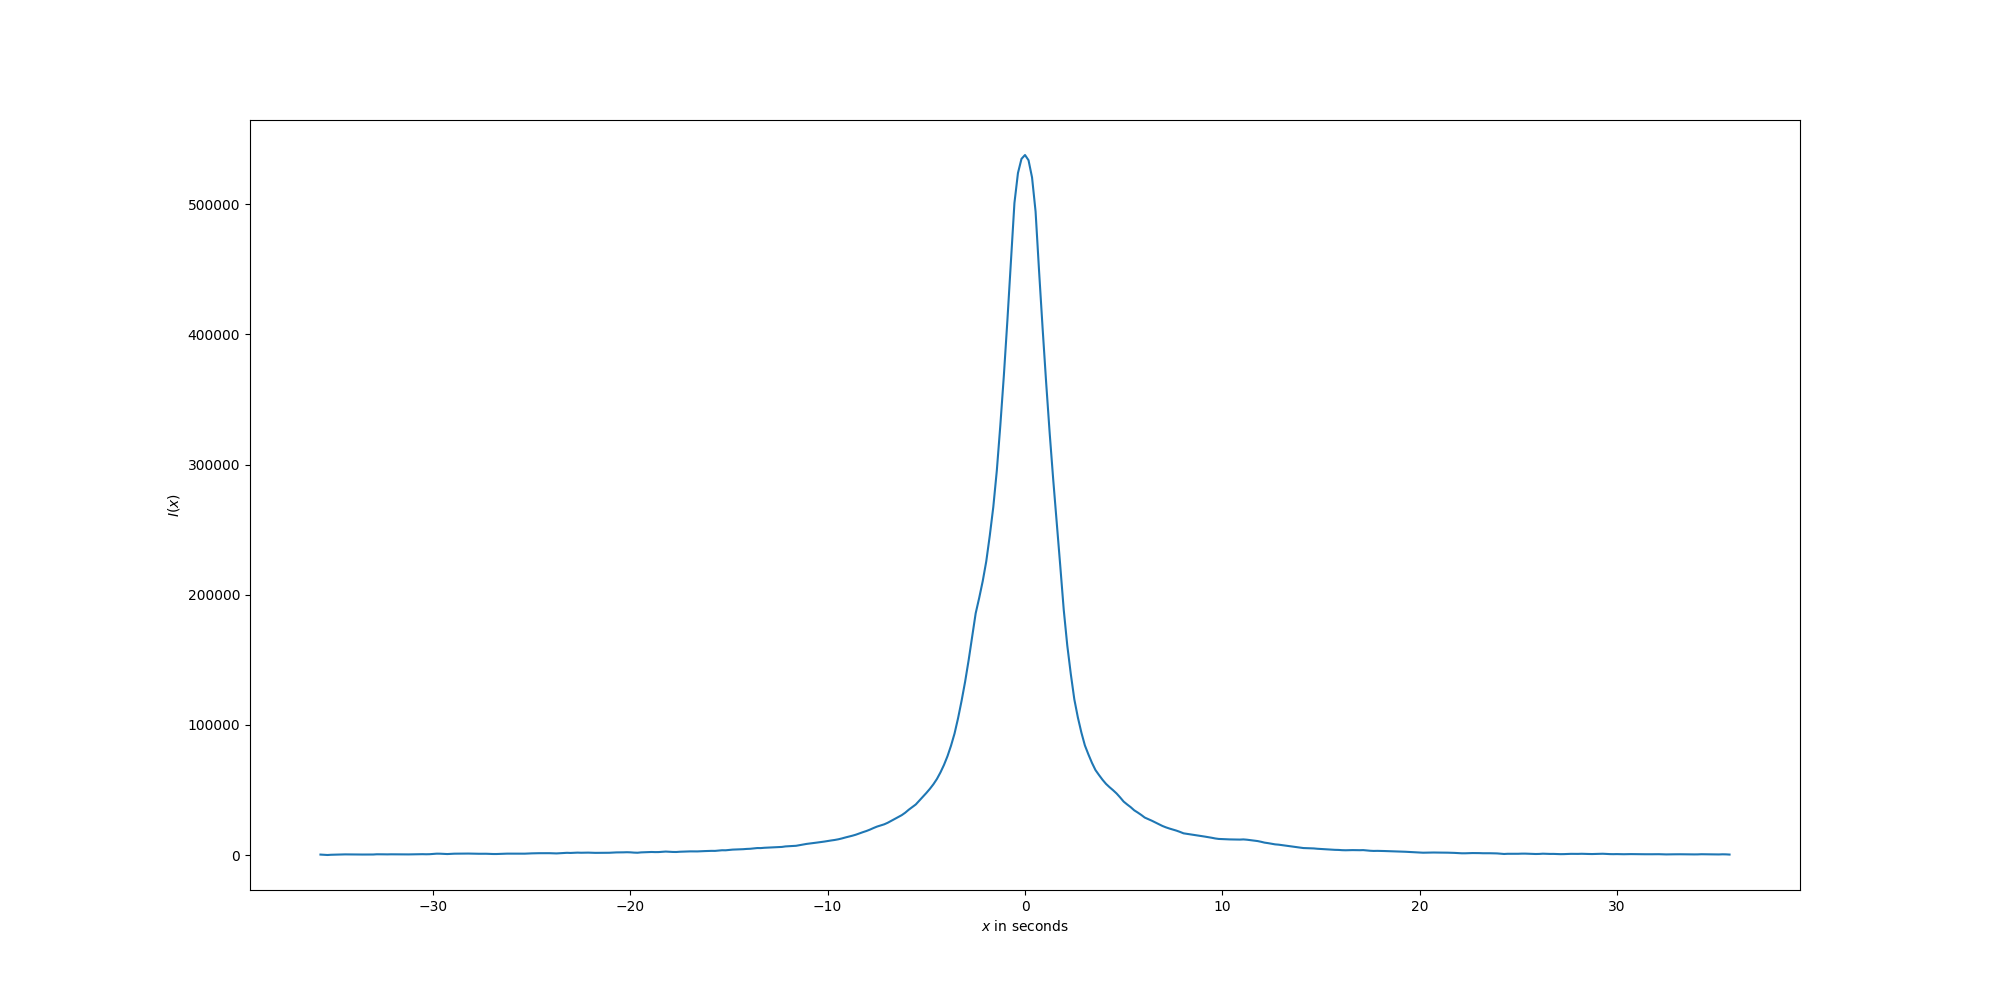
\includegraphics[width = 0.8\textwidth]{R_slice_min.png}
			\caption{Срез потока по направлению, вдоль которого профиль наименьший. Фильтр R}
		\end{figure}
		\begin{figure}
		\centering
			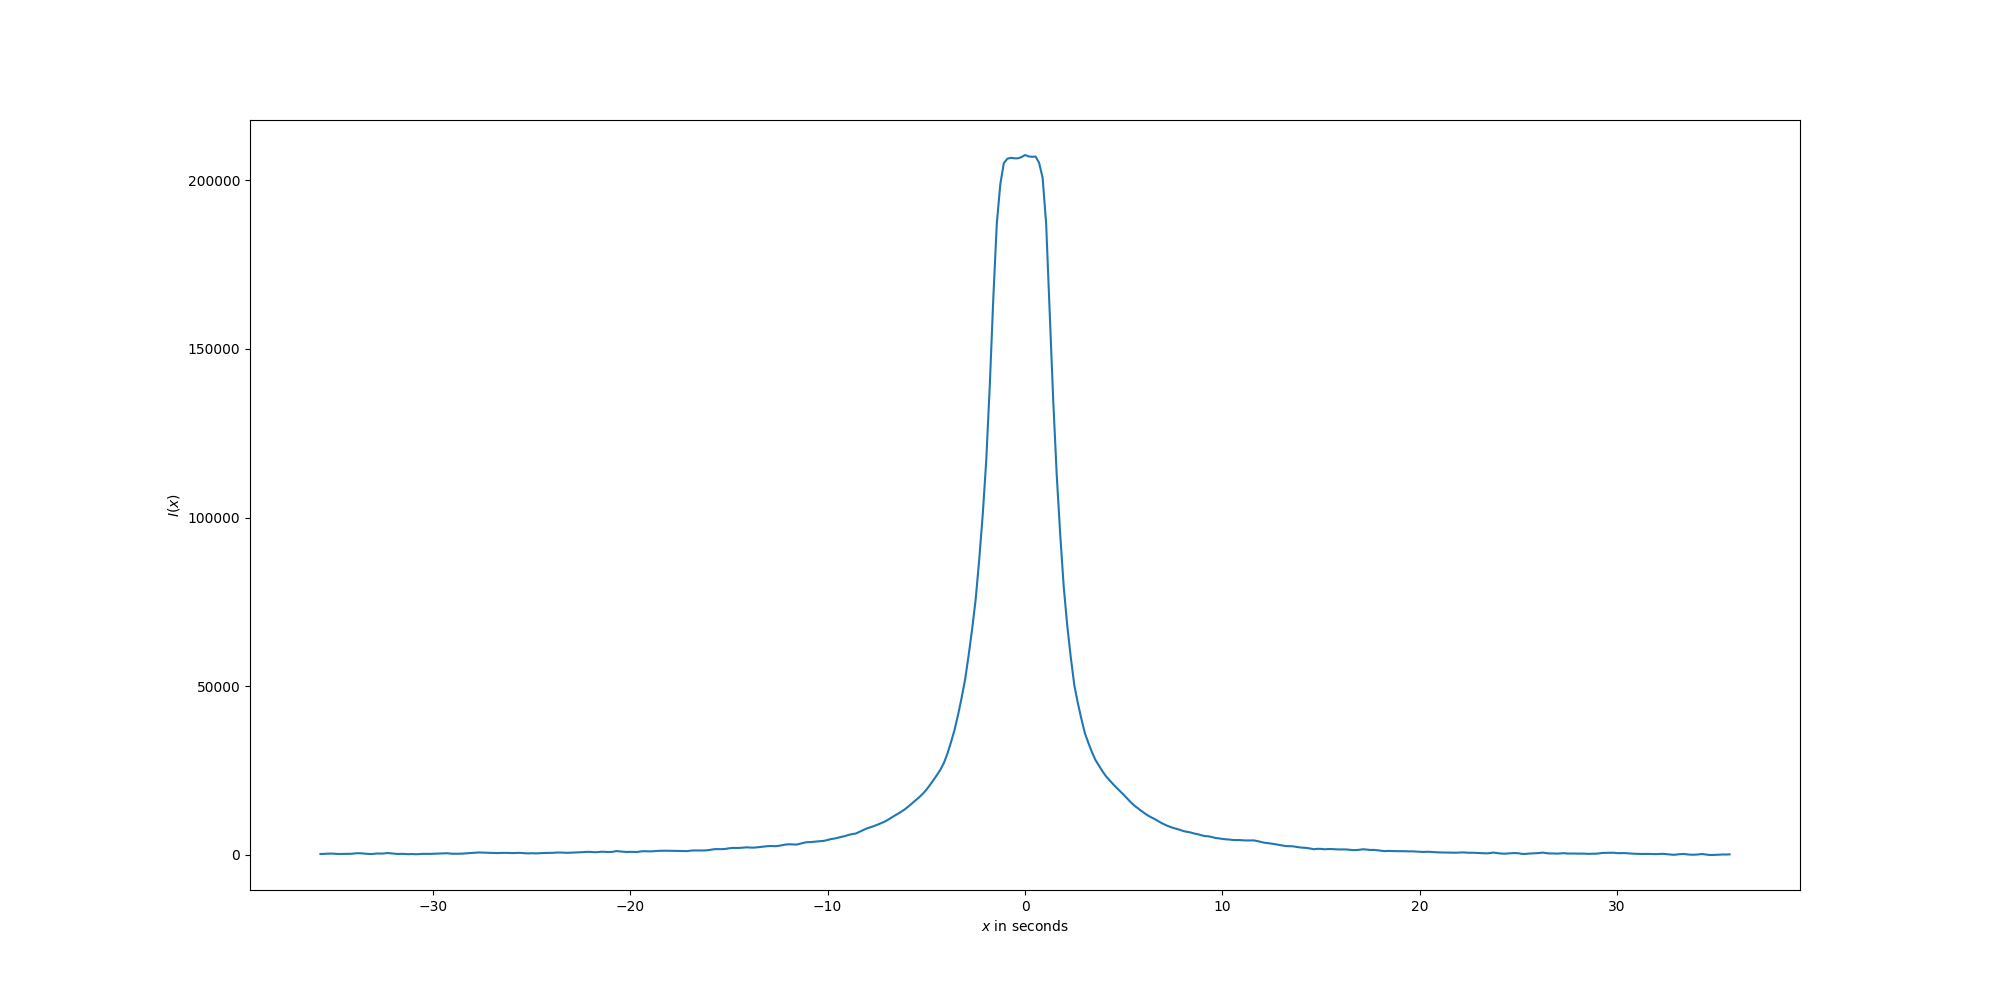
\includegraphics[width = 0.8\textwidth]{I_slice_min.png}
						\caption{Срез потока по направлению, вдоль которого профиль наименьший. Фильтр I}
		\end{figure}
		\begin{figure}
		\centering
			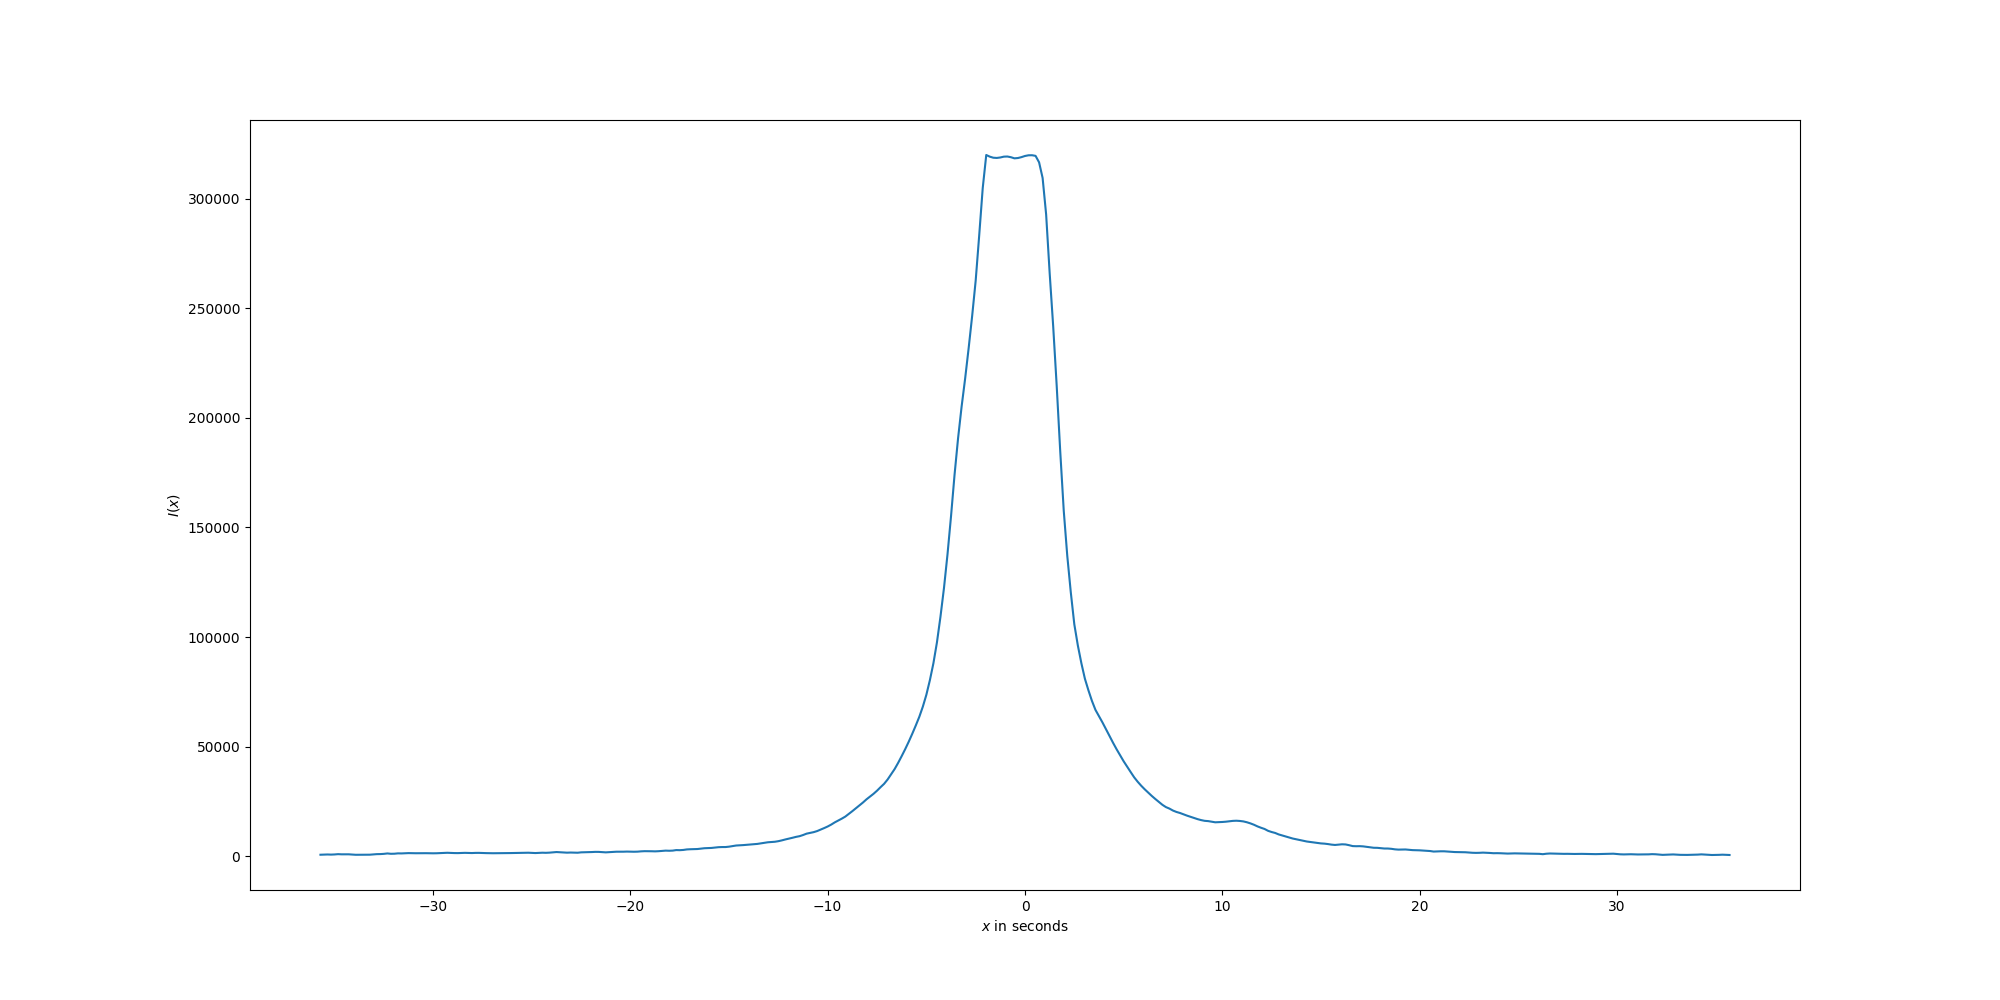
\includegraphics[width = 0.8\textwidth]{B_slice_min.png}
						\caption{Срез потока по направлению, вдоль которого профиль наименьший. Фильтр B}
					\end{figure}
		\begin{figure}
		\centering
			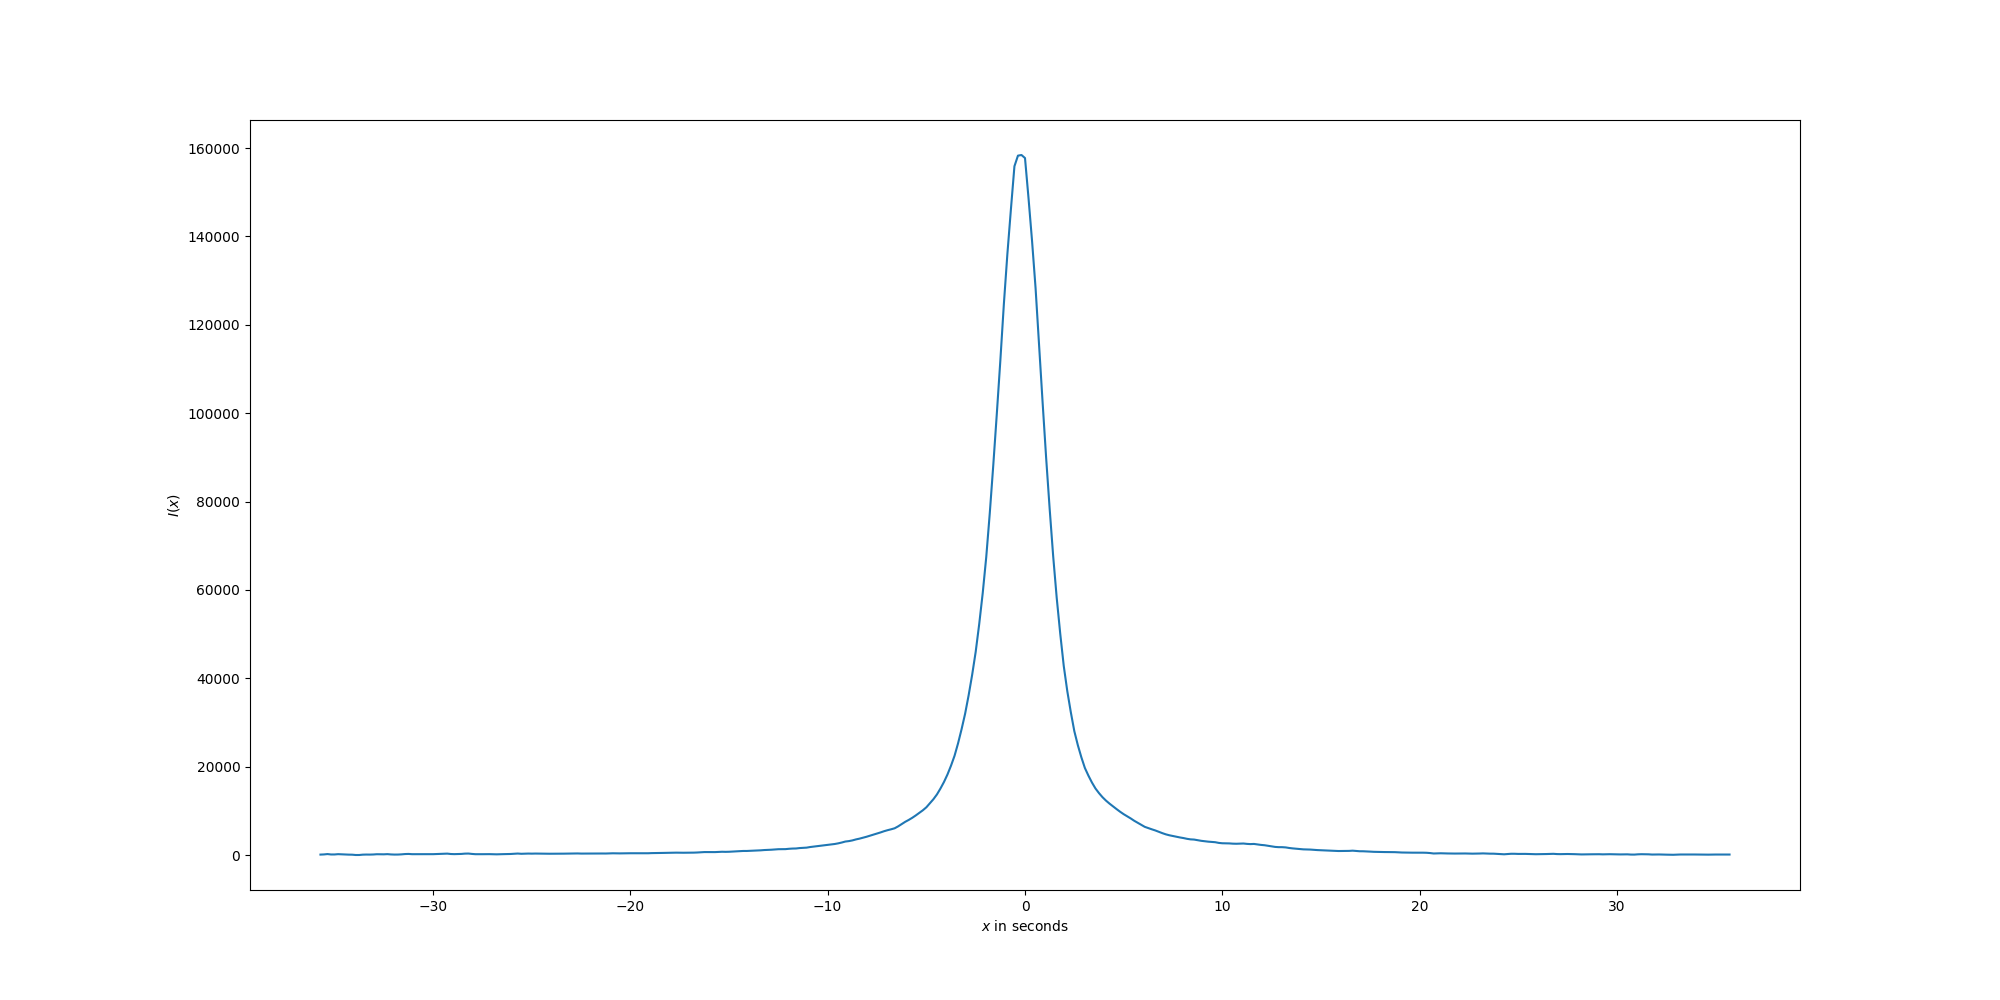
\includegraphics[width = 0.8\textwidth]{V_slice_min.png}
			\caption{Срез потока по направлению, вдоль которого профиль наименьший. Фильтр V}
\end{figure}
\begin{figure}
		\centering
			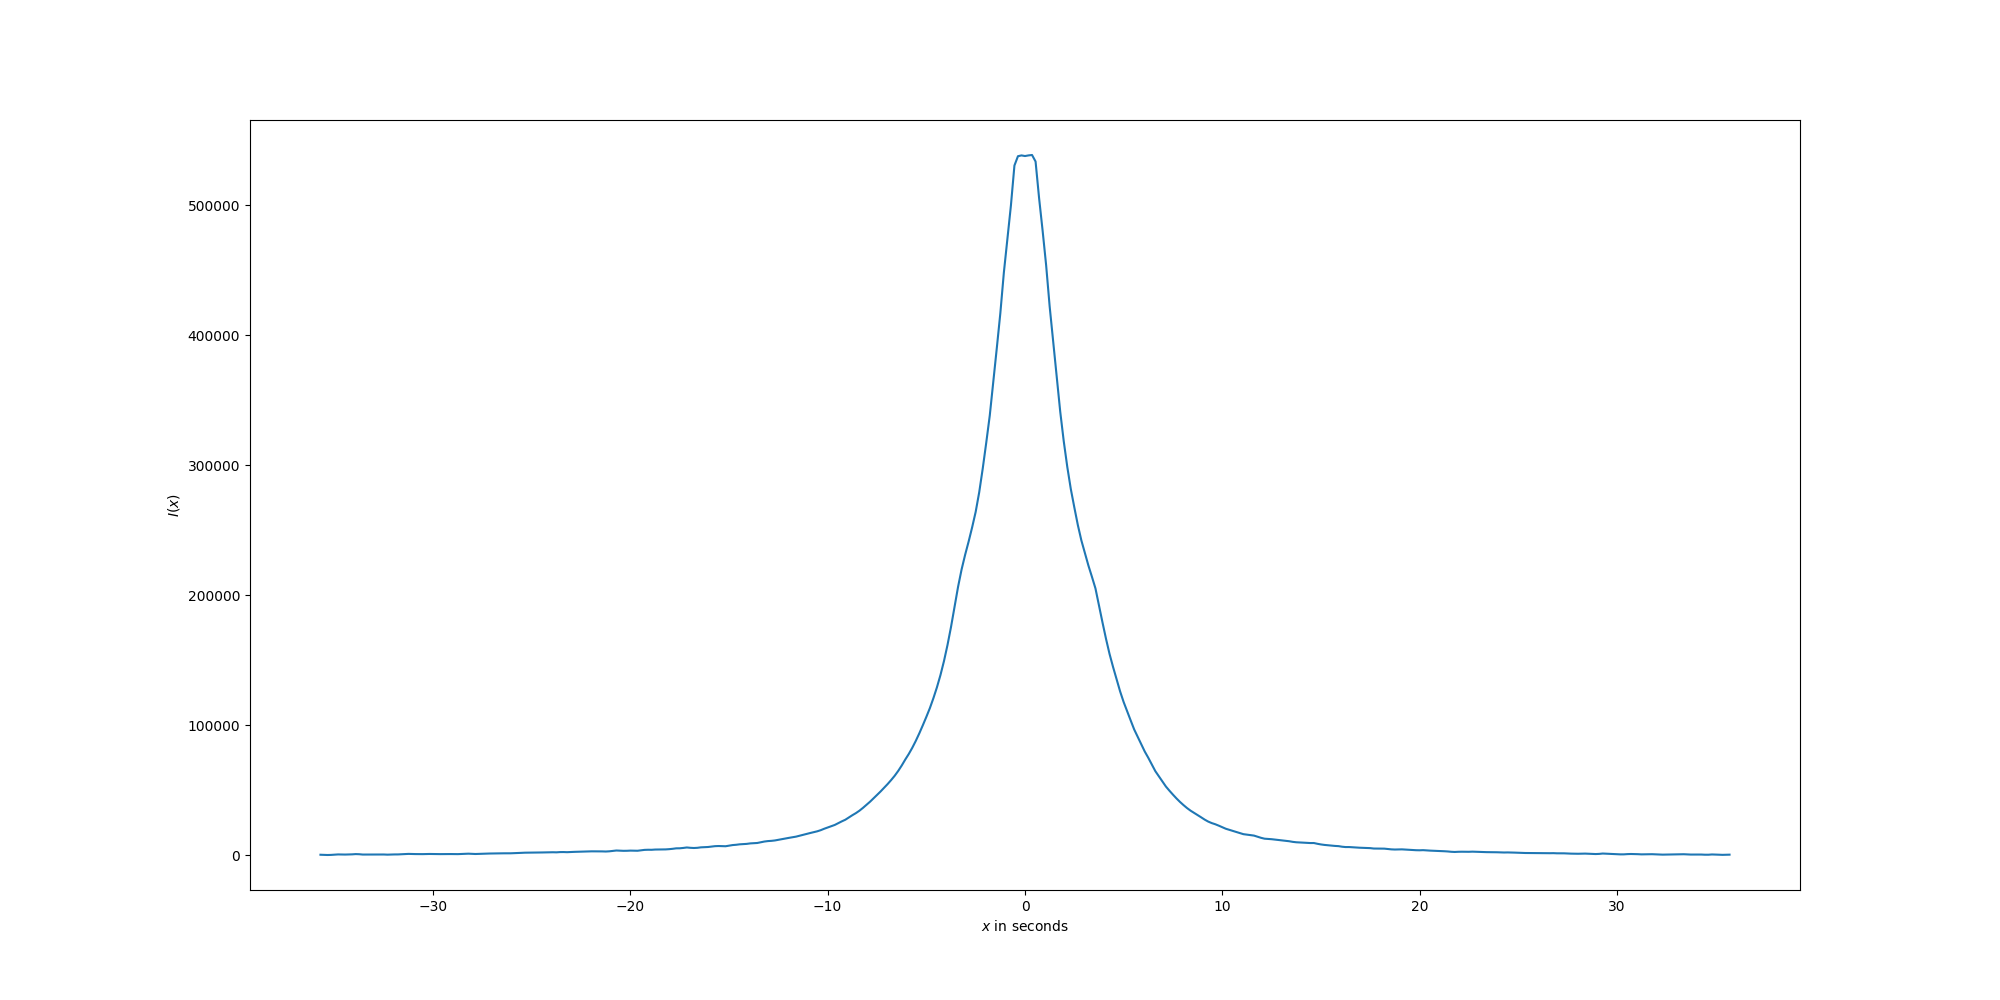
\includegraphics[width = 0.8\textwidth]{R_slice_max.png}
			\caption{Срез потока по направлению, вдоль которого профиль наибольший. Фильтр R}
		\end{figure}
		\begin{figure}
		\centering
			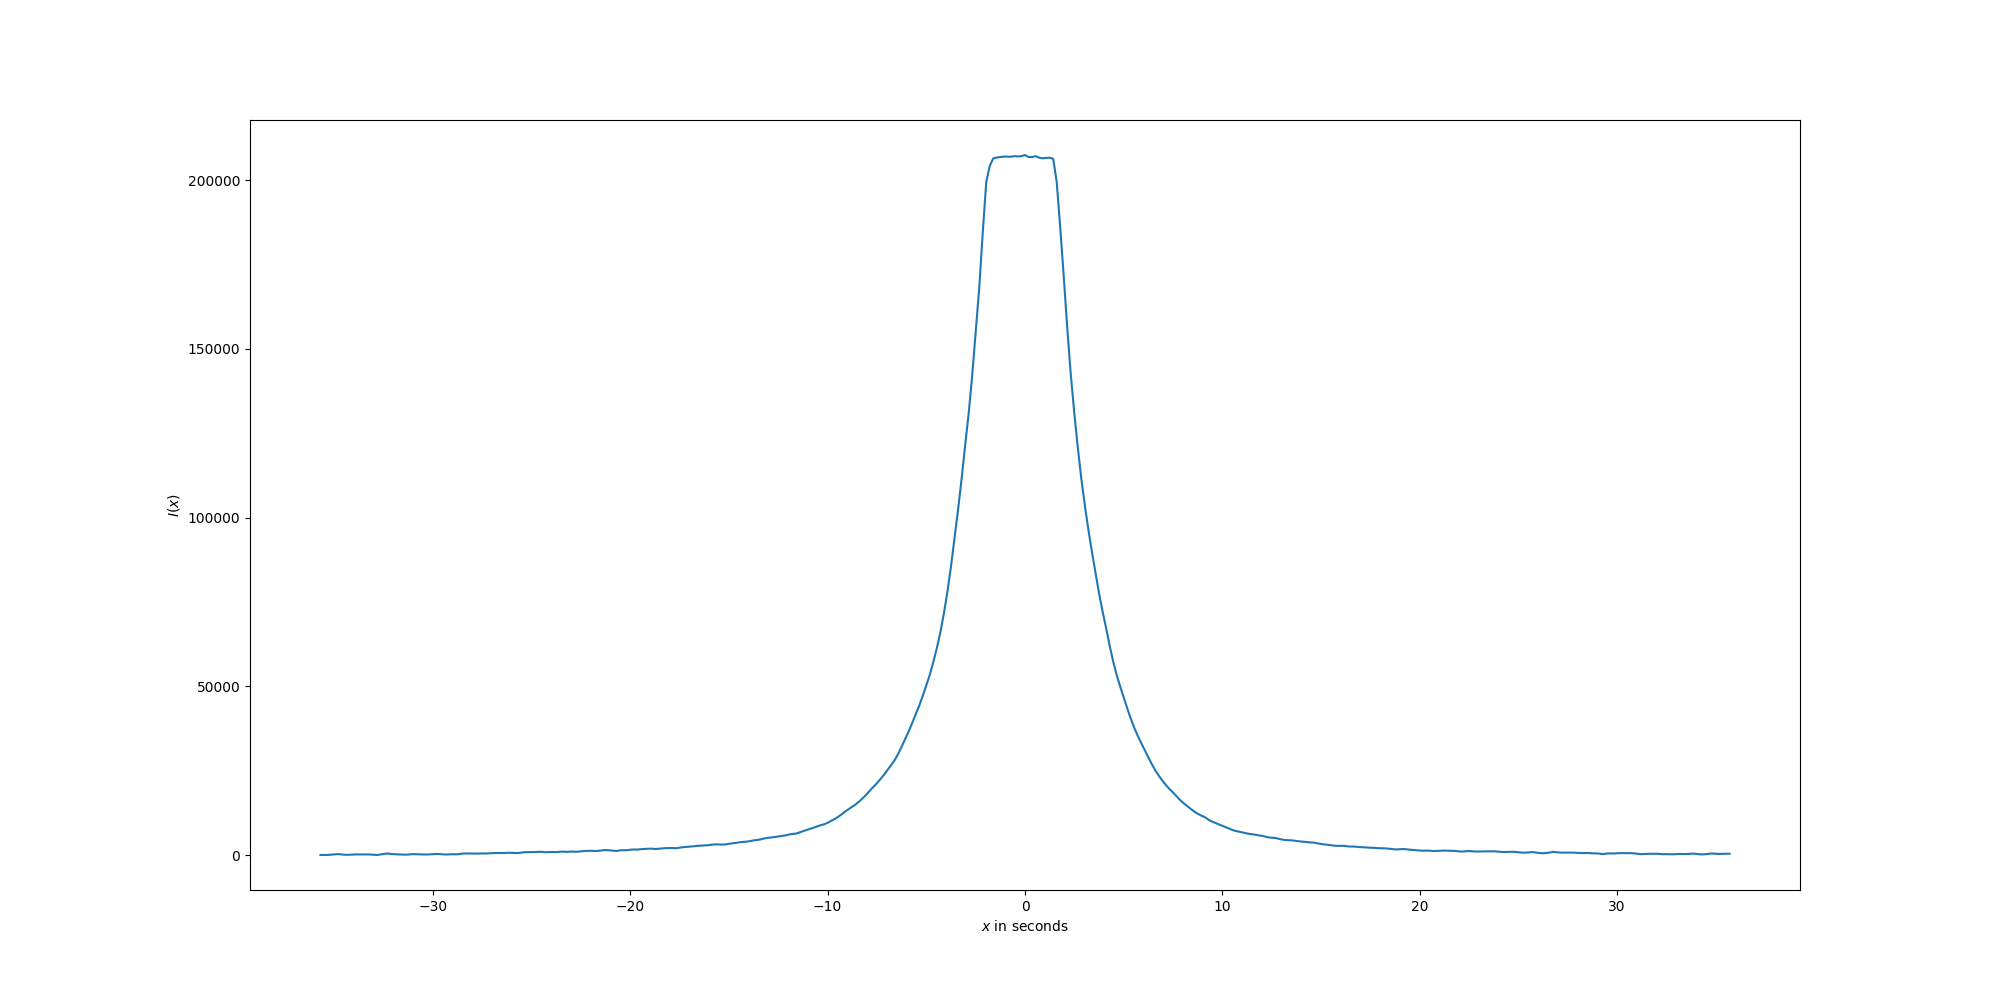
\includegraphics[width = 0.8\textwidth]{I_slice_max.png}
						\caption{Срез потока по направлению, вдоль которого профиль наибольший. Фильтр I}
		\end{figure}
		\begin{figure}
		\centering
			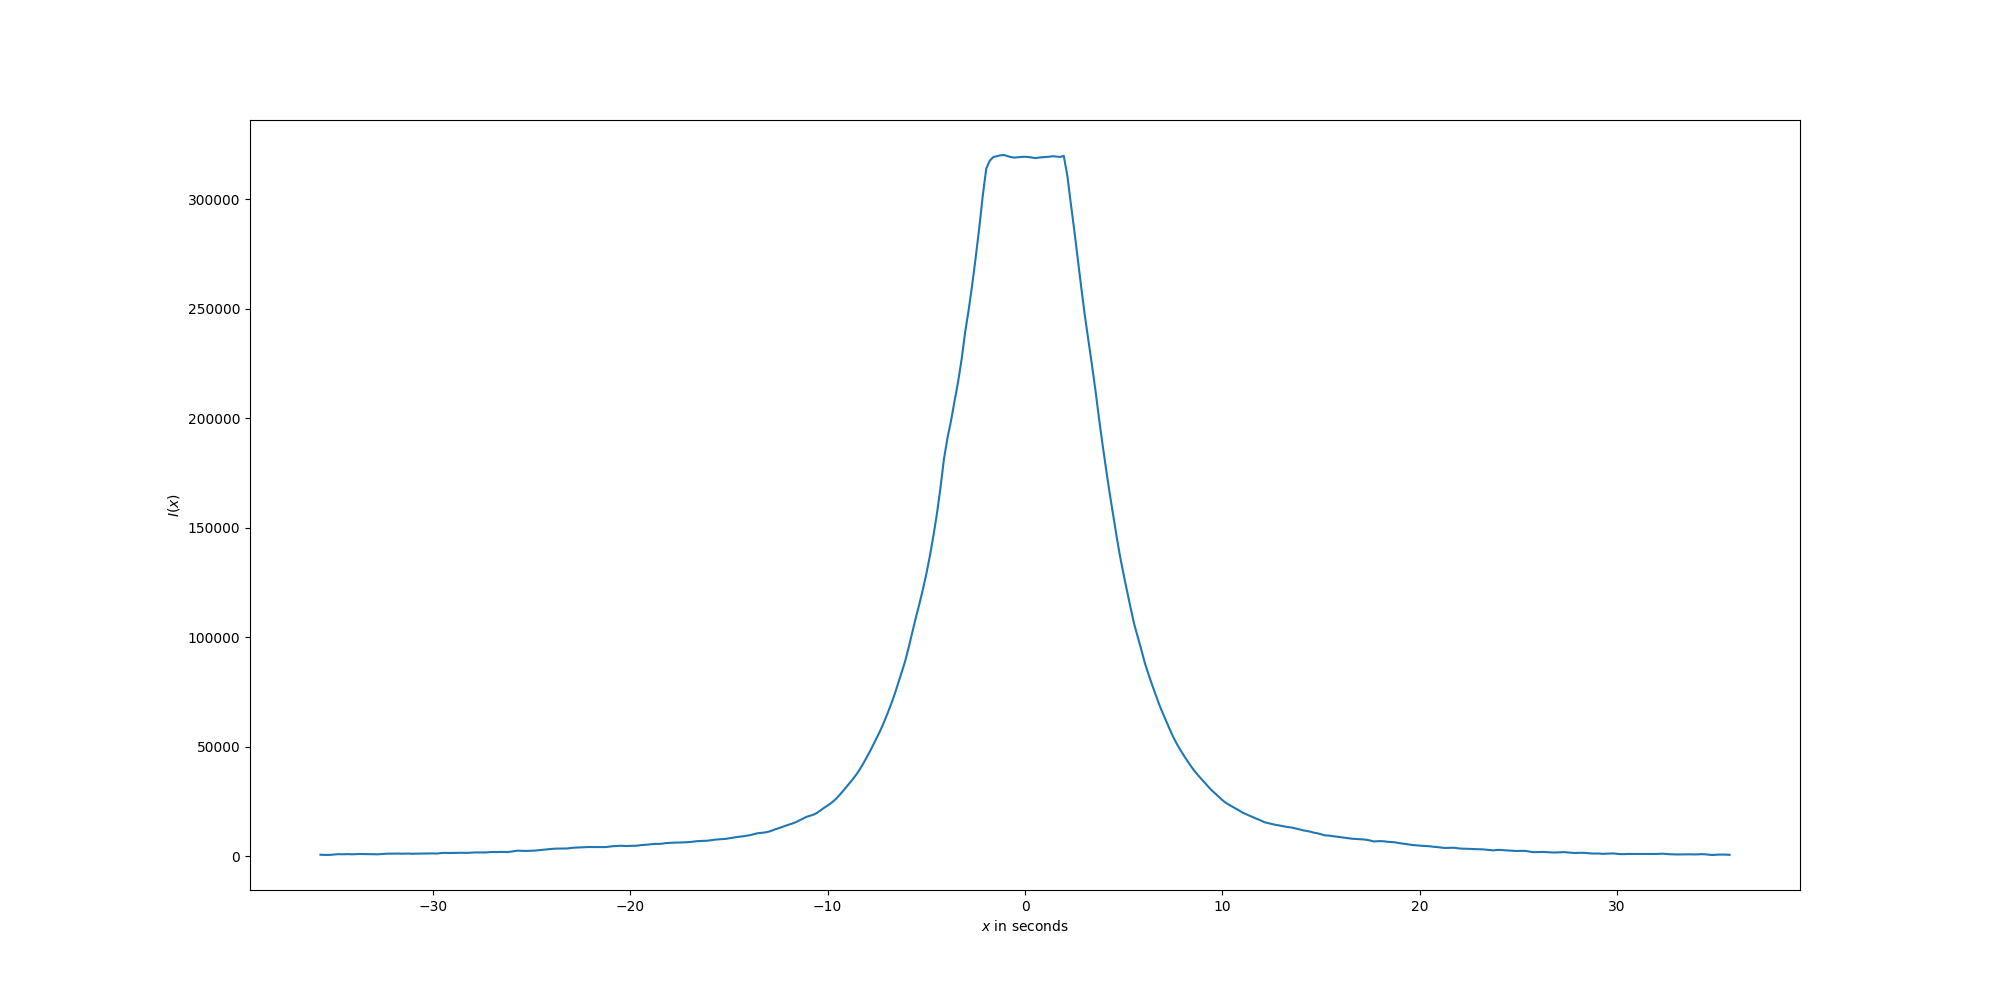
\includegraphics[width = 0.8\textwidth]{B_slice_max.png}
						\caption{Срез потока по направлению, вдоль которого профиль наибольший. Фильтр B}
					\end{figure}
		\begin{figure}
		\centering
			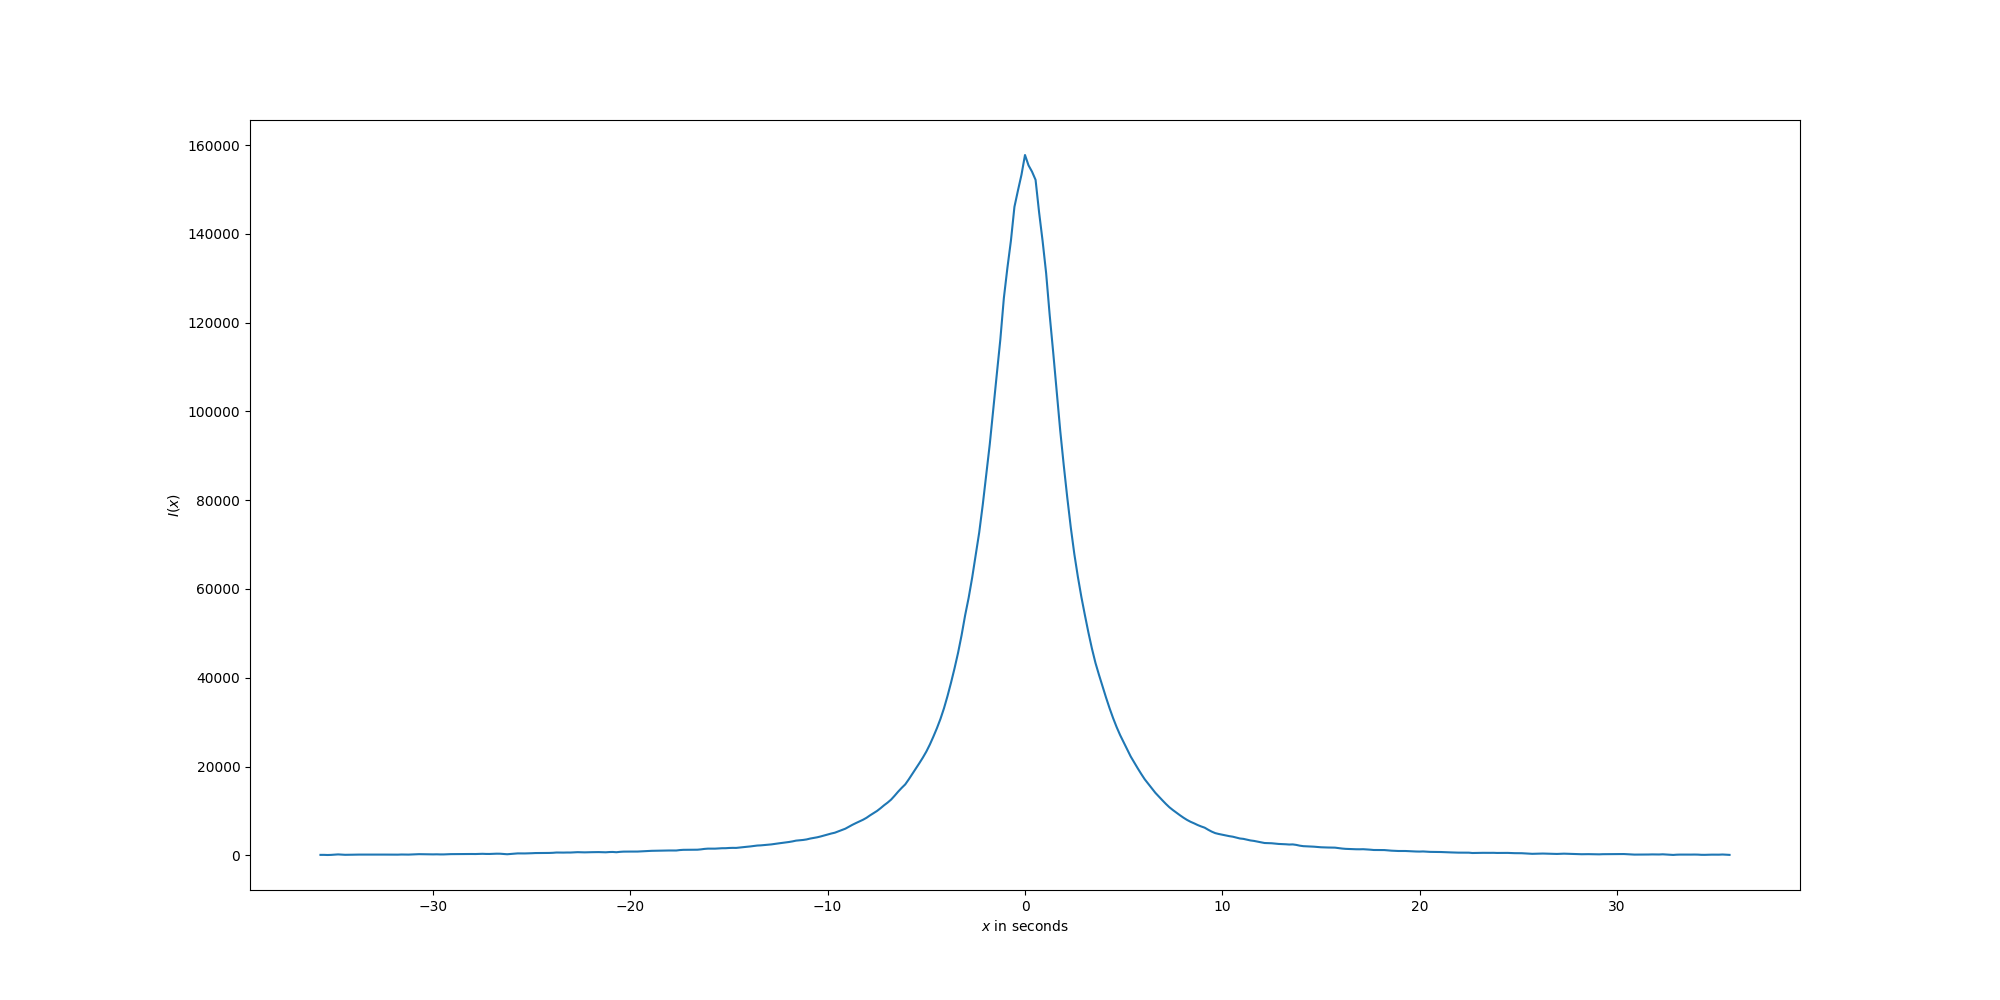
\includegraphics[width = 0.8\textwidth]{V_slice_max.png}
			\caption{Срез потока по направлению, вдоль которого профиль наименьший. Фильтр V}
\end{figure}
\end{document}